\documentclass{standalone}
\usepackage{tikz}
\begin{document}


\tikzset{every picture/.style={line width=0.75pt}} %set default line width to 0.75pt

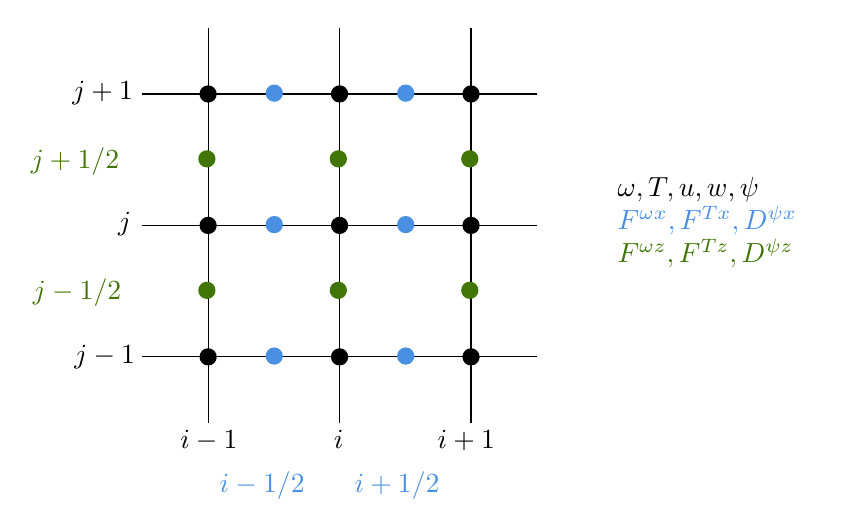
\begin{tikzpicture}[x=0.75pt,y=0.75pt,yscale=-1,xscale=1]
%uncomment if require: \path (0,460); %set diagram left start at 0, and has height of 460

%Shape: Grid [id:dp5156694921663176]
\draw  [draw opacity=0] (160,350) -- (160,160) -- (350,160) -- (350,350) -- cycle ; \draw   (160,318.33) -- (350,318.33)(160,255) -- (350,255)(160,191.67) -- (350,191.67) ; \draw   (191.67,350) -- (191.67,160)(255,350) -- (255,160)(318.33,350) -- (318.33,160) ; \draw    ;
%Shape: Ellipse [id:dp2883513131329054]
\draw  [draw opacity=0][fill={rgb, 255:red, 0; green, 0; blue, 0 }  ,fill opacity=1 ] (314.18,191.67) .. controls (314.18,189.37) and (316.04,187.51) .. (318.33,187.51) .. controls (320.63,187.51) and (322.49,189.37) .. (322.49,191.67) .. controls (322.49,193.96) and (320.63,195.82) .. (318.33,195.82) .. controls (316.04,195.82) and (314.18,193.96) .. (314.18,191.67) -- cycle ;
%Shape: Ellipse [id:dp04421815579196142]
\draw  [draw opacity=0][fill={rgb, 255:red, 0; green, 0; blue, 0 }  ,fill opacity=1 ] (250.84,191.67) .. controls (250.84,189.37) and (252.7,187.51) .. (255,187.51) .. controls (257.3,187.51) and (259.16,189.37) .. (259.16,191.67) .. controls (259.16,193.96) and (257.3,195.82) .. (255,195.82) .. controls (252.7,195.82) and (250.84,193.96) .. (250.84,191.67) -- cycle ;
%Shape: Ellipse [id:dp8134726969276163]
\draw  [draw opacity=0][fill={rgb, 255:red, 0; green, 0; blue, 0 }  ,fill opacity=1 ] (187.51,191.67) .. controls (187.51,189.37) and (189.37,187.51) .. (191.67,187.51) .. controls (193.96,187.51) and (195.82,189.37) .. (195.82,191.67) .. controls (195.82,193.96) and (193.96,195.82) .. (191.67,195.82) .. controls (189.37,195.82) and (187.51,193.96) .. (187.51,191.67) -- cycle ;
%Shape: Circle [id:dp6447008244671211]
\draw  [draw opacity=0][fill={rgb, 255:red, 0; green, 0; blue, 0 }  ,fill opacity=1 ] (314.18,255) .. controls (314.18,252.7) and (316.04,250.84) .. (318.33,250.84) .. controls (320.63,250.84) and (322.49,252.7) .. (322.49,255) .. controls (322.49,257.3) and (320.63,259.16) .. (318.33,259.16) .. controls (316.04,259.16) and (314.18,257.3) .. (314.18,255) -- cycle ;
%Shape: Circle [id:dp4047596541546261]
\draw  [draw opacity=0][fill={rgb, 255:red, 0; green, 0; blue, 0 }  ,fill opacity=1 ] (250.84,255) .. controls (250.84,252.7) and (252.7,250.84) .. (255,250.84) .. controls (257.3,250.84) and (259.16,252.7) .. (259.16,255) .. controls (259.16,257.3) and (257.3,259.16) .. (255,259.16) .. controls (252.7,259.16) and (250.84,257.3) .. (250.84,255) -- cycle ;
%Shape: Circle [id:dp32813091137594075]
\draw  [draw opacity=0][fill={rgb, 255:red, 0; green, 0; blue, 0 }  ,fill opacity=1 ] (187.51,255) .. controls (187.51,252.7) and (189.37,250.84) .. (191.67,250.84) .. controls (193.96,250.84) and (195.82,252.7) .. (195.82,255) .. controls (195.82,257.3) and (193.96,259.16) .. (191.67,259.16) .. controls (189.37,259.16) and (187.51,257.3) .. (187.51,255) -- cycle ;
%Shape: Ellipse [id:dp817925558887048]
\draw  [draw opacity=0][fill={rgb, 255:red, 0; green, 0; blue, 0 }  ,fill opacity=1 ] (314.18,318.33) .. controls (314.18,316.04) and (316.04,314.18) .. (318.33,314.18) .. controls (320.63,314.18) and (322.49,316.04) .. (322.49,318.33) .. controls (322.49,320.63) and (320.63,322.49) .. (318.33,322.49) .. controls (316.04,322.49) and (314.18,320.63) .. (314.18,318.33) -- cycle ;
%Shape: Ellipse [id:dp8656185087649877]
\draw  [draw opacity=0][fill={rgb, 255:red, 0; green, 0; blue, 0 }  ,fill opacity=1 ] (250.84,318.33) .. controls (250.84,316.04) and (252.7,314.18) .. (255,314.18) .. controls (257.3,314.18) and (259.16,316.04) .. (259.16,318.33) .. controls (259.16,320.63) and (257.3,322.49) .. (255,322.49) .. controls (252.7,322.49) and (250.84,320.63) .. (250.84,318.33) -- cycle ;
%Shape: Ellipse [id:dp48374861067766384]
\draw  [draw opacity=0][fill={rgb, 255:red, 0; green, 0; blue, 0 }  ,fill opacity=1 ] (187.51,318.33) .. controls (187.51,316.04) and (189.37,314.18) .. (191.67,314.18) .. controls (193.96,314.18) and (195.82,316.04) .. (195.82,318.33) .. controls (195.82,320.63) and (193.96,322.49) .. (191.67,322.49) .. controls (189.37,322.49) and (187.51,320.63) .. (187.51,318.33) -- cycle ;
%Shape: Ellipse [id:dp4309901930879714]
\draw  [draw opacity=0][fill={rgb, 255:red, 74; green, 144; blue, 226 }  ,fill opacity=1 ] (282.71,191.27) .. controls (282.71,188.98) and (284.57,187.11) .. (286.86,187.11) .. controls (289.16,187.11) and (291.02,188.98) .. (291.02,191.27) .. controls (291.02,193.57) and (289.16,195.43) .. (286.86,195.43) .. controls (284.57,195.43) and (282.71,193.57) .. (282.71,191.27) -- cycle ;
%Shape: Ellipse [id:dp15821066359758507]
\draw  [draw opacity=0][fill={rgb, 255:red, 74; green, 144; blue, 226 }  ,fill opacity=1 ] (219.38,191.27) .. controls (219.38,188.98) and (221.24,187.11) .. (223.53,187.11) .. controls (225.83,187.11) and (227.69,188.98) .. (227.69,191.27) .. controls (227.69,193.57) and (225.83,195.43) .. (223.53,195.43) .. controls (221.24,195.43) and (219.38,193.57) .. (219.38,191.27) -- cycle ;
%Shape: Circle [id:dp13316183014085148]
\draw  [draw opacity=0][fill={rgb, 255:red, 74; green, 144; blue, 226 }  ,fill opacity=1 ] (282.71,254.6) .. controls (282.71,252.31) and (284.57,250.45) .. (286.86,250.45) .. controls (289.16,250.45) and (291.02,252.31) .. (291.02,254.6) .. controls (291.02,256.9) and (289.16,258.76) .. (286.86,258.76) .. controls (284.57,258.76) and (282.71,256.9) .. (282.71,254.6) -- cycle ;
%Shape: Circle [id:dp47632222781043554]
\draw  [draw opacity=0][fill={rgb, 255:red, 74; green, 144; blue, 226 }  ,fill opacity=1 ] (219.38,254.6) .. controls (219.38,252.31) and (221.24,250.45) .. (223.53,250.45) .. controls (225.83,250.45) and (227.69,252.31) .. (227.69,254.6) .. controls (227.69,256.9) and (225.83,258.76) .. (223.53,258.76) .. controls (221.24,258.76) and (219.38,256.9) .. (219.38,254.6) -- cycle ;
%Shape: Circle [id:dp3131527955633957]
\draw  [draw opacity=0][fill={rgb, 255:red, 74; green, 144; blue, 226 }  ,fill opacity=1 ] (282.71,317.94) .. controls (282.71,315.64) and (284.57,313.78) .. (286.86,313.78) .. controls (289.16,313.78) and (291.02,315.64) .. (291.02,317.94) .. controls (291.02,320.23) and (289.16,322.09) .. (286.86,322.09) .. controls (284.57,322.09) and (282.71,320.23) .. (282.71,317.94) -- cycle ;
%Shape: Circle [id:dp8092704894784628]
\draw  [draw opacity=0][fill={rgb, 255:red, 74; green, 144; blue, 226 }  ,fill opacity=1 ] (219.38,317.94) .. controls (219.38,315.64) and (221.24,313.78) .. (223.53,313.78) .. controls (225.83,313.78) and (227.69,315.64) .. (227.69,317.94) .. controls (227.69,320.23) and (225.83,322.09) .. (223.53,322.09) .. controls (221.24,322.09) and (219.38,320.23) .. (219.38,317.94) -- cycle ;
%Shape: Circle [id:dp39304804596774257]
\draw  [draw opacity=0][fill={rgb, 255:red, 65; green, 117; blue, 5 }  ,fill opacity=1 ] (313.58,222.94) .. controls (313.58,220.64) and (315.44,218.78) .. (317.74,218.78) .. controls (320.04,218.78) and (321.9,220.64) .. (321.9,222.94) .. controls (321.9,225.23) and (320.04,227.09) .. (317.74,227.09) .. controls (315.44,227.09) and (313.58,225.23) .. (313.58,222.94) -- cycle ;
%Shape: Circle [id:dp5888433740705601]
\draw  [draw opacity=0][fill={rgb, 255:red, 65; green, 117; blue, 5 }  ,fill opacity=1 ] (250.25,222.94) .. controls (250.25,220.64) and (252.11,218.78) .. (254.41,218.78) .. controls (256.7,218.78) and (258.56,220.64) .. (258.56,222.94) .. controls (258.56,225.23) and (256.7,227.09) .. (254.41,227.09) .. controls (252.11,227.09) and (250.25,225.23) .. (250.25,222.94) -- cycle ;
%Shape: Circle [id:dp7331962928037836]
\draw  [draw opacity=0][fill={rgb, 255:red, 65; green, 117; blue, 5 }  ,fill opacity=1 ] (186.92,222.94) .. controls (186.92,220.64) and (188.78,218.78) .. (191.07,218.78) .. controls (193.37,218.78) and (195.23,220.64) .. (195.23,222.94) .. controls (195.23,225.23) and (193.37,227.09) .. (191.07,227.09) .. controls (188.78,227.09) and (186.92,225.23) .. (186.92,222.94) -- cycle ;
%Shape: Circle [id:dp8789269682274454]
\draw  [draw opacity=0][fill={rgb, 255:red, 65; green, 117; blue, 5 }  ,fill opacity=1 ] (313.58,286.27) .. controls (313.58,283.98) and (315.44,282.11) .. (317.74,282.11) .. controls (320.04,282.11) and (321.9,283.98) .. (321.9,286.27) .. controls (321.9,288.57) and (320.04,290.43) .. (317.74,290.43) .. controls (315.44,290.43) and (313.58,288.57) .. (313.58,286.27) -- cycle ;
%Shape: Circle [id:dp4838671839917066]
\draw  [draw opacity=0][fill={rgb, 255:red, 65; green, 117; blue, 5 }  ,fill opacity=1 ] (250.25,286.27) .. controls (250.25,283.98) and (252.11,282.11) .. (254.41,282.11) .. controls (256.7,282.11) and (258.56,283.98) .. (258.56,286.27) .. controls (258.56,288.57) and (256.7,290.43) .. (254.41,290.43) .. controls (252.11,290.43) and (250.25,288.57) .. (250.25,286.27) -- cycle ;
%Shape: Circle [id:dp8118114867489652]
\draw  [draw opacity=0][fill={rgb, 255:red, 65; green, 117; blue, 5 }  ,fill opacity=1 ] (186.92,286.27) .. controls (186.92,283.98) and (188.78,282.11) .. (191.07,282.11) .. controls (193.37,282.11) and (195.23,283.98) .. (195.23,286.27) .. controls (195.23,288.57) and (193.37,290.43) .. (191.07,290.43) .. controls (188.78,290.43) and (186.92,288.57) .. (186.92,286.27) -- cycle ;


% Text Node
\draw (381,228.4) node [anchor=north west][inner sep=0.75pt]    {$ \begin{array}{l}
\omega ,T,u,w,\psi \\
\textcolor[rgb]{0.29,0.56,0.89}{F}\textcolor[rgb]{0.29,0.56,0.89}{^{\omega x}}\textcolor[rgb]{0.29,0.56,0.89}{,F}\textcolor[rgb]{0.29,0.56,0.89}{^{Tx} ,D^{\psi x}}\\
\textcolor[rgb]{0.25,0.46,0.02}{F}\textcolor[rgb]{0.25,0.46,0.02}{^{\omega z}}\textcolor[rgb]{0.25,0.46,0.02}{,F}\textcolor[rgb]{0.25,0.46,0.02}{^{Tz} ,D^{\psi z}}
\end{array}$};
% Text Node
\draw (251,352.4) node [anchor=north west][inner sep=0.75pt]    {$i$};
% Text Node
\draw (261,372.4) node [anchor=north west][inner sep=0.75pt]  [color={rgb, 255:red, 74; green, 144; blue, 226 }  ,opacity=1 ]  {$i+1/2$};
% Text Node
\draw (301,352.4) node [anchor=north west][inner sep=0.75pt]    {$i+1$};
% Text Node
\draw (177,352.4) node [anchor=north west][inner sep=0.75pt]    {$i-1$};
% Text Node
\draw (196,372.4) node [anchor=north west][inner sep=0.75pt]  [color={rgb, 255:red, 74; green, 144; blue, 226 }  ,opacity=1 ]  {$i-1/2$};
% Text Node
\draw (147,247.4) node [anchor=north west][inner sep=0.75pt]    {$j$};
% Text Node
\draw (126,311.4) node [anchor=north west][inner sep=0.75pt]    {$j-1$};
% Text Node
\draw (125,184.4) node [anchor=north west][inner sep=0.75pt]    {$j+1$};
% Text Node
\draw (105,216.4) node [anchor=north west][inner sep=0.75pt]  [color={rgb, 255:red, 65; green, 117; blue, 5 }  ,opacity=1 ]  {$j+1/2$};
% Text Node
\draw (106,279.4) node [anchor=north west][inner sep=0.75pt]  [color={rgb, 255:red, 65; green, 117; blue, 5 }  ,opacity=1 ]  {$j-1/2$};


\end{tikzpicture}

\end{document}